% ==============================================================================
%  A Latency-Aware Pure Black-Box UQ Benchmark for LLMs  (G x D -> M -> V)
%  ACL-format. Requires acl.sty + acl_natbib.bst (see README.md).
%  Compile:  pdflatex main ; bibtex main ; pdflatex main ; pdflatex main
% ==============================================================================
\documentclass[11pt]{article}
\usepackage[review]{acl}
% FALLBACK: comment the line above, uncomment below, if acl.sty is missing.
% \usepackage[margin=1in]{geometry}\usepackage{natbib}\bibliographystyle{plainnat}

\usepackage{times}
\usepackage{latexsym}
\usepackage[T1]{fontenc}
\usepackage[utf8]{inputenc}
\usepackage{microtype}
\usepackage{booktabs}
\usepackage{amsmath}
\usepackage{amssymb}
\usepackage{multirow}
\usepackage{graphicx}
\usepackage{xcolor}
\usepackage{url}
\usepackage{enumitem}
\usepackage{pgfplots}
\pgfplotsset{compat=1.17}
\usepgfplotslibrary{groupplots}

\newcommand{\best}[1]{\textbf{#1}}
\newcommand{\grey}[1]{\textcolor{gray}{#1}}

\title{$G\times D\to M\to V$: A Latency-Aware, Pure Black-Box \\
Uncertainty-Quantification Benchmark for Language Models}

% author block omitted: [review] mode emits "Anonymous ACL submission".
% CAMERA-READY: restore \author{...} here.
\begin{document}
\maketitle

\begin{abstract}
Uncertainty quantification (UQ) for large language models is evaluated in fragmented
conditions: different papers assume white-box logits or black-box text, use one target
model and a handful of datasets, and---almost universally---ignore the \emph{cost} of
producing the uncertainty signal. We present a unified benchmark organized around four
explicit axes, $G$ (generator/target), $D$ (dataset), $M$ (UQ/truth method), and $V$
(evaluation metric), with two design commitments that existing suites lack: (i)
\textbf{pure black-box} semantics enforced at the interface---methods see the target's
\emph{text} only, and any method that reads target log-probabilities (e.g.\ P(True)) is
labelled grey-box and reported separately; and (ii) \textbf{latency measured relative to
the target}, making the accuracy--cost trade a first-class result rather than a
footnote. We instantiate the benchmark with four frontier targets (open Qwen3-32B and
Llama-3.3-70B; closed GPT-4o and Claude-Haiku-4.5), seven task domains, and $\sim$70
method configurations spanning sampling-consistency, graph-spectral, verbalized, and
\emph{distilled-proxy} families, each swept over sample budgets $N\in\{1,3,5,10\}$ and
scored with eight calibration/ranking metrics plus a latency frontier. A single cached,
content-hashed generation per $(G,D)$ guarantees that every method is compared on
identical inputs. Across 3{,}000+ method$\times$dataset$\times$target evaluations we find
that (a) the best method is \emph{generator-dependent} (graph-spectral and verbalized
confidence tie on Qwen at $\approx$0.65; verbalized confidence leads on Llama at 0.664 AUROC,
where semantic entropy falls to near-chance); (b)
sampling-consistency methods are \emph{uninformative at $N{=}1$} (AUROC $0.500$) and need
$N{=}10$ samples---i.e.\ ten target generations---to peak; and (c) distilled proxies
reach competitive AUROC at a \emph{target-decoupled} $\sim$25--45\,ms, hundreds of times
below any sampling method. We release the harness, caches, and all configurations.
\end{abstract}

% ==============================================================================
\section{Introduction}
% ==============================================================================
When a deployed system relies on a language model it does not control, it needs a signal
for \emph{when the model is wrong}. The research literature on LLM uncertainty
quantification is rich but hard to compare across: methods are proposed under different
access assumptions (logits vs.\ text), evaluated on different single targets, on
non-overlapping datasets, and---most consequentially for deployment---\emph{without
reporting how much compute the uncertainty signal costs}. A method that needs ten extra
generations of a 70B model to reach its headline AUROC is not comparable, at a system
level, to one that needs a single small forward pass, yet current tables place them side
by side on accuracy alone.

We argue that a useful UQ benchmark must make three things explicit and enforceable:
the \emph{access level} of each method (so ``black-box'' is a guarantee, not a claim),
the \emph{four axes} that a UQ result actually depends on, and the \emph{latency}
relative to the target. We organize the benchmark as
\[
  G \;\times\; D \;\longrightarrow\; M \;\longrightarrow\; V,
\]
where the generator $G$ and dataset $D$ define a cached evaluation surface, each method
$M$ maps a target's text to an uncertainty score, and each metric $V$ scores that against
correctness. This paper describes the benchmark, its harness, and a large comprehensive
sweep, and reports the cross-axis phenomena that only a unified suite can
surface.\footnote{Harness, configurations, cached results, and scripts:
\url{[repository URL withheld for anonymous review]}}

\paragraph{Contributions.}
\begin{enumerate}[leftmargin=1.4em,itemsep=1pt,topsep=2pt]
\item A \textbf{pure black-box, latency-aware UQ benchmark} with enforced access levels,
four explicit axes, and a cached content-hashed harness that guarantees identical inputs
across methods and sample budgets (\S\ref{sec:design}).
\item A \textbf{comprehensive instantiation}: 4 frontier targets $\times$ 7 domains
$\times$ $\sim$70 method configurations (sampling-consistency, graph-spectral, verbalized,
distilled-proxy, and a grey-box P(True) reference) $\times$ 8 metrics, with sample-budget
sweeps and measured latency (\S\ref{sec:results}).
\item \textbf{Cross-axis findings} a single-condition study cannot see: strong
generator-dependence of the best method, the sample-budget scaling wall of
consistency methods, and a distinct fast frontier occupied by distilled proxies
(\S\ref{sec:results}, \S\ref{sec:latency}).
\end{enumerate}

% ==============================================================================
\section{Related Benchmarks}
% ==============================================================================
Prior UQ evaluations fall into three groups. \emph{White-box} suites assume access to
the target's logits or hidden states and evaluate perplexity, energy, or evidential
scores; these do not apply to hosted APIs. \emph{Black-box, single-target} studies
introduce sampling-consistency \citep{kuhn2023semantic,farquhar2024detecting} and
graph-spectral \citep{lin2023generating} methods, or verbalized confidence
\citep{lin2022teaching}, but usually on one model and a few datasets, and---critically---%
report accuracy without the number of target calls the method consumes. \emph{Library}
efforts such as \textsc{TruthTorchLM} \citep{bakman2024truthtorchlm} unify method
\emph{implementations} but not an access-enforced, latency-first \emph{evaluation}
protocol. Our benchmark contributes the protocol: explicit axes, an enforced pure
black-box interface with grey-box methods flagged, sample-budget sweeps, and
target-relative latency as a reported axis.

% ==============================================================================
\section{Benchmark Design}\label{sec:design}
% ==============================================================================
\subsection{Axis $G$: Generators (targets)}
Targets span scale and provider: open-weights \textbf{Qwen3-32B}
\citep{yang2024qwen3} and \textbf{Llama-3.3-70B} \citep{dubey2024llama3}, and closed
frontier \textbf{GPT-4o} and \textbf{Claude-Haiku-4.5} accessed through a text-only
gateway. The harness is generator-agnostic; adding a target is a registry entry mapping a
friendly key to a provider-qualified id, backend, and \emph{access level}. Access levels
are verified, not assumed: a helper probes each provider to confirm it returns text only
before any ``black-box'' result is recorded.

\subsection{Axis $D$: Datasets}
Seven categories, one representative dataset each, 150 items per cell:
General (TriviaQA \citealp{joshi2017triviaqa}), Medical-open (BioASQ
\citealp{tsatsaronis2015bioasq}), Medical-MCQ (MedQA \citealp{jin2021medqa}),
Medical-long-form (MedLFQA), Math (GSM8K \citealp{cobbe2021gsm8k}), Adversarial
(TruthfulQA \citealp{lin2021truthfulqa}), and Factual (Wikipedia). The categories span
the axes UQ practitioners care about: answer format (free-form / MCQ / numeric),
knowledge type (general / specialist), and failure mode (recall error vs.\ imitative
falsehood). The harness supports a broader roster (open-domain QA, MMLU-medical, and
others) behind the same interface. Labels use an LLM judge, with exact-match on
multiple-choice.

\subsection{Axis $M$: Methods}
The method roster (Table~\ref{tab:roster}) is deliberately comprehensive and organized by
family and \emph{access level}. Sampling-consistency and graph-spectral methods read a
set of $N$ target samples and summarize their semantic dispersion; verbalized confidence
elicits one self-reported score; distilled proxies read the logits of a small white-box
student distilled from the target's text. P(True) is included but \emph{labelled
grey-box}---it reads the target's probability of the token ``true''---and is never
counted as a pure-BB result. Full mathematical definitions of every family---semantic-set
and graph-spectral consistency scores, the nine proxy read-outs (including the evidential
AU/EU head), and the DALD/DisAAD/Ours training objectives---are in
Appendix~\ref{app:methods}. Every consistency method is swept over sample budgets
$N\in\{1,3,5,10\}$ by \emph{truncating} the same cached samples, so the $N$-sweep costs no
extra generation and is perfectly controlled.

\begin{table}[t]\centering\small
\setlength{\tabcolsep}{3pt}
\begin{tabular}{p{3.5cm} c c}
\toprule
family (\# configs) & access & target calls\\
\midrule
Graph-spectral: Eccentricity, MatrixDegree, EigV, SumEigen (Conf/Unc) $\times N$ & black-box & $N$\\
Semantic-set: DiscreteSemEntropy, NumSemanticSet, KernelLangEntropy $\times N$ & black-box & $N$\\
Similarity: LexicalSimilarity $\times N$ & black-box & $N$\\
Verbalized confidence & black-box & $1$\\
\textbf{Distilled proxy}: DALD, DisAAD, Ours $\times$ 9 read-outs & black-box & $0$\\
\grey{P(True) (reference)} & \grey{grey-box} & \grey{$1$}\\
\bottomrule
\end{tabular}
\caption{Method roster by family, access level, and \emph{target-call cost}. Proxies pay
zero target calls at inference (one small student forward); consistency methods pay $N$;
verbalized/P(True) pay one. $\sim$70 total configurations.}
\label{tab:roster}
\end{table}

\subsection{Axis $V$: Metrics}
Each method is scored with a ranking/calibration suite: AUROC (primary), AUPRC, AUARC,
prediction-rejection ratio (PRR), and calibration error (ECE/ACE/MCE) and Brier score,
all against binary answer correctness, aggregated as mean$\pm$std over seeds. Orthogonal
to $V$ is the \emph{latency frontier}: p50 wall-clock of the uncertainty computation
under a fixed protocol (\S\ref{sec:latency}). We report AUROC in the main tables and the
full suite in the release.

\subsection{Harness}
The pipeline runs in four stages. \textbf{A} generates and \emph{caches} the target's
answers (and $N$ samples) once per $(G,D)$, keyed by a content hash over dataset,
generator, decoding, budget, and size, so a decoding change never silently reuses a stale
cache. \textbf{B} labels with the judge. \textbf{C} scores every method by \emph{reading
the same cache} (sweeping $N$ by truncation). \textbf{D} evaluates $V$ and the latency
frontier. This ``generate once, score many'' discipline is what makes the comparison
fair and the $N$-sweep exact.

% ==============================================================================
\section{Comprehensive Results}\label{sec:results}
% ==============================================================================
Table~\ref{tab:leaderboard} is the benchmark's central artifact: per-dataset AUROC for
representative methods of each family on the two open targets, at each method's best
sample budget. Two cross-axis phenomena stand out.

\begin{table*}[t]\centering\small
\setlength{\tabcolsep}{4pt}
\begin{tabular}{l ccccccc c}
\toprule
method & trivia & bioasq & medqa & medlfqa & gsm8k & truthful & wiki & \best{MEAN}\\
\midrule
\multicolumn{9}{l}{\emph{Target: Qwen3-32B}}\\
Verbalized conf.\ ($N{=}1$)       & \best{0.728} & \grey{--} & \best{0.702} & \grey{--} & 0.668 & \best{0.686} & 0.483 & 0.653\\
Eccentricity ($N{=}10$)           & 0.817 & \grey{--} & 0.522 & \grey{--} & 0.764 & 0.607 & 0.564 & \best{0.655}\\
Semantic entropy ($N{=}10$)       & \best{0.819} & \grey{--} & 0.500 & \grey{--} & 0.710 & 0.557 & 0.533 & 0.624\\
Lexical similarity ($N{=}10$)     & 0.695 & \grey{--} & 0.539 & \grey{--} & 0.575 & 0.501 & \best{0.607} & 0.583\\
Distilled proxy ($N{=}0$)         & 0.618 & \grey{--} & 0.705 & \grey{--} & 0.780 & 0.472 & 0.593 & 0.634\\
\grey{P(True) (grey-box)}         & \grey{0.827} & \grey{--} & \grey{0.690} & \grey{--} & \grey{\best{0.838}} & \grey{0.623} & \grey{0.560} & \grey{0.708}\\
\midrule
\multicolumn{9}{l}{\emph{Target: Llama-3.3-70B}}\\
Verbalized conf.\ ($N{=}1$)       & 0.656 & \grey{--} & \best{0.699} & \best{0.648} & 0.627 & \best{0.797} & \best{0.557} & \best{0.664}\\
Eccentricity ($N{=}10$)           & \best{0.796} & \grey{--} & 0.585 & 0.653 & 0.702 & 0.500 & 0.526 & 0.627\\
Semantic entropy ($N{=}10$)       & 0.630 & \grey{--} & 0.496 & 0.501 & 0.585 & 0.473 & 0.492 & 0.529\\
Lexical similarity ($N{=}10$)     & 0.758 & \grey{--} & 0.667 & 0.456 & 0.591 & 0.518 & 0.544 & 0.589\\
Distilled proxy ($N{=}0$)         & 0.631 & \grey{--} & 0.600 & 0.450 & 0.694 & 0.551 & 0.507 & 0.572\\
\grey{P(True) (grey-box)}         & \grey{0.690} & \grey{--} & \grey{0.549} & \grey{0.567} & \grey{0.711} & \grey{0.564} & \grey{0.535} & \grey{0.603}\\
\bottomrule
\end{tabular}
\caption{Per-dataset AUROC leaderboard, representative method per family, best sample
budget, two open targets. Distilled proxy is the best deployable proxy read via
perplexity. Grey rows are grey-box (read target log-probs) and excluded from the pure-BB
ranking. \textbf{Cells whose minority class is $<15$ are excluded} (``--'') and dropped from the
means, since an AUROC there is undefined or set by one or two items. This removes BioASQ on both
targets ($150/150$ correct on Qwen, $149/150$ on Llama) and MedLFQA on Qwen ($139/150$). On
Llama, BioASQ would otherwise contribute $0.97$--$1.00$ and inflate every mean by $0.04$--$0.06$.
Means are consequently over five datasets (Qwen) and six (Llama) and are not directly
comparable across the two blocks. No undefined cell is imputed as $0.500$. Per-cell class
balances are in Appendix~\ref{app:details}.}
\label{tab:leaderboard}
\end{table*}

\paragraph{The best method is generator-dependent.} On Qwen3-32B graph-spectral and verbalized
confidence are \emph{statistically indistinguishable} at the top (Eccentricity 0.655 vs.\
verbalized 0.653, a gap far inside the $\pm0.045$ standard error at $n{\approx}150$); on
Llama-3.3-70B \emph{verbalized confidence leads} (0.664) ahead of the same graph-spectral
method (0.627), with semantic entropy \emph{collapsing} to near-chance (0.529). The
generator-dependence is therefore asymmetric: it is a real reordering on Llama, and a tie on
Qwen. Recall that these two means are over different dataset sets (five vs.\ six) after
degenerate-cell exclusion, so we compare methods \emph{within} a target, never across. The closed targets sharpen this (Appendix~\ref{app:closed}): verbalized
confidence is the strongest method on \emph{both} GPT-4o (0.737) and Claude-Haiku (0.672),
and on Haiku it is the \emph{only} method above chance---every sampling-consistency method
there is at or below 0.55. So verbalized confidence wins on three of four targets and
graph-spectral on the fourth (Qwen): no single method wins across targets, and a benchmark
reporting one generator would draw the opposite conclusion depending on which it picked---%
exactly the fragmentation the $G$ axis exposes.

\paragraph{Domain structure is sharp and method-specific.} Verbalized confidence is
strong on Adversarial (TruthfulQA: Llama 0.797) where consistency is
\emph{structurally blind} (Eccentricity 0.500---imitative falsehoods are produced
consistently), while consistency methods dominate General/Math where sample dispersion
tracks error. This complementarity is only visible with the full $D\times M$ grid.

\begin{table}[t]\centering\small
\setlength{\tabcolsep}{4pt}
\begin{tabular}{l cccc}
\toprule
family (mean AUROC) & $N{=}1$ & $N{=}3$ & $N{=}5$ & $N{=}10$\\
\midrule
\multicolumn{5}{l}{\emph{Qwen3-32B}}\\
Eccentricity      & 0.500 & 0.628 & 0.645 & \best{0.655}\\
SumEigen / EigV   & 0.500 & 0.619 & 0.633 & \best{0.651}\\
Semantic entropy  & 0.500 & 0.578 & 0.599 & \best{0.624}\\
Lexical sim.      & 0.500 & 0.563 & 0.571 & \best{0.583}\\
Verbalized conf.  & \best{0.653} & 0.653 & 0.653 & 0.653\\
\midrule
\multicolumn{5}{l}{\emph{Llama-3.3-70B}}\\
Eccentricity      & 0.500 & 0.584 & 0.617 & \best{0.627}\\
Lexical sim.      & 0.500 & \best{0.596} & 0.592 & 0.589\\
Semantic entropy  & 0.500 & 0.515 & 0.520 & \best{0.529}\\
Verbalized conf.  & \best{0.664} & 0.664 & 0.664 & 0.664\\
\bottomrule
\end{tabular}
\caption{Sample-budget ($N$) scaling. Consistency/graph methods are \emph{uninformative
at $N{=}1$} (AUROC 0.500---one sample has no dispersion) and require $N{=}10$ target
generations to peak. Verbalized confidence is $N$-invariant (one call). The distilled
proxy (not shown; $N{=}0$) reaches 0.61--0.63 with no target samples at all.}
\label{tab:nsweep}
\end{table}

\begin{figure}[t]
\centering
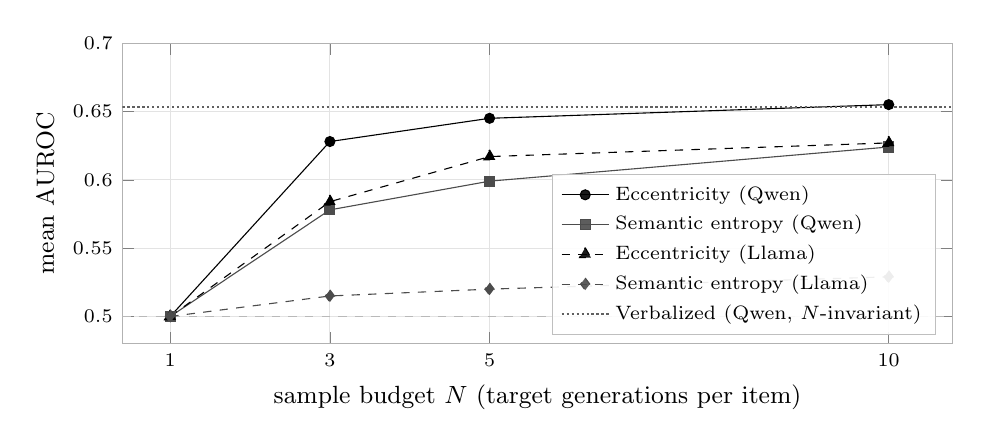
\begin{tikzpicture}
\begin{axis}[
  width=\columnwidth, height=5.4cm,
  xlabel={sample budget $N$ (target generations per item)},
  ylabel={mean AUROC},
  xtick={1,3,5,10}, xmin=0.4, xmax=10.8, ymin=0.48, ymax=0.70,
  xlabel style={font=\small}, ylabel style={font=\small},
  tick label style={font=\scriptsize},
  grid=major, grid style={gray!22}, axis line style={gray!60},
  legend style={font=\scriptsize, at={(0.98,0.03)}, anchor=south east,
                draw=gray!50, fill=white, fill opacity=0.9, text opacity=1},
  legend cell align=left,
]
% chance line
\addplot[gray!55, dashed, forget plot] coordinates {(0.4,0.5) (10.8,0.5)};
% Qwen3-32B
\addplot[mark=*, mark size=1.8pt, black] coordinates {(1,0.500)(3,0.628)(5,0.645)(10,0.655)};
\addlegendentry{Eccentricity (Qwen)}
\addplot[mark=square*, mark size=1.8pt, gray!60!black]
  coordinates {(1,0.500)(3,0.578)(5,0.599)(10,0.624)};
\addlegendentry{Semantic entropy (Qwen)}
% Llama-3.3-70B
\addplot[mark=triangle*, mark size=2.4pt, black, dashed]
  coordinates {(1,0.500)(3,0.584)(5,0.617)(10,0.627)};
\addlegendentry{Eccentricity (Llama)}
\addplot[mark=diamond*, mark size=2.2pt, gray!60!black, dashed]
  coordinates {(1,0.500)(3,0.515)(5,0.520)(10,0.529)};
\addlegendentry{Semantic entropy (Llama)}
% verbalized confidence: budget-invariant, one call
\addplot[densely dotted, thick, gray!75!black, no marks]
  coordinates {(0.4,0.653)(10.8,0.653)};
\addlegendentry{Verbalized (Qwen, $N$-invariant)}
\end{axis}
\end{tikzpicture}
\caption{\textbf{Sample budget is a hidden cost.} Every dispersion-based method is pinned at
AUROC $0.500$ at $N{=}1$---a single sample has no dispersion, so this is definitional, not
empirical---and climbs only as the system pays more target generations, peaking at $N{=}10$.
Verbalized confidence (dotted) is budget-invariant at one call, and distilled proxies (not
shown) sit at $N{=}0$. Semantic entropy also illustrates the generator effect: it is
competitive on Qwen and near chance on Llama at every budget. Means are over non-degenerate
cells (Table~\ref{tab:leaderboard}).}
\label{fig:nsweep}
\end{figure}

\paragraph{Sample budget is a hidden cost.} Table~\ref{tab:nsweep} and Fig.~\ref{fig:nsweep} make the
accuracy--budget dependence explicit. Every consistency/graph method scores exactly
$0.500$ at $N{=}1$---a single sample has no dispersion to measure---and climbs to its
peak only at $N{=}10$, i.e.\ ten target generations per item. Verbalized confidence is
budget-invariant, and distilled proxies need \emph{zero} target samples. This axis is
invisible in tables that fix $N$.

\paragraph{Ranking is not calibration.} AUROC alone hides two effects
(Table~\ref{tab:metrics}). First, \emph{AUPRC is base-rate inflated}: because correct
answers dominate, every method scores $0.82$--$0.92$ AUPRC regardless of how well it
ranks errors, so AUPRC is a poor discriminator here. Second, the
\emph{prediction--rejection ratio} (PRR)---the useful secondary ranking metric---adds
granularity that AUROC misses: LexicalSimilarity on Qwen ranks non-trivially by AUROC
(0.571) but has PRR $0.067$, i.e.\ rejecting by its score barely beats random rejection.
Calibration metrics (ECE/ACE/MCE/Brier) are computed and released, but the raw
uncertainty scores are not probabilities, so cross-method ECE is only meaningful after
per-method calibration (natively-probabilistic verbalized confidence and P(True) reach
ECE $\approx 0.14$; the un-normalized graph and LogTokU-proxy scores do not, by construction).
We therefore report the three scale-robust ranking metrics in the main text and the full
eight-metric suite in the release.

\begin{table}[t]\centering\small
\setlength{\tabcolsep}{4pt}
\begin{tabular}{l ccc}
\toprule
method (mean over datasets) & AUROC & AUPRC & PRR\\
\midrule
\multicolumn{4}{l}{\emph{Qwen3-32B}}\\
Verbalized conf.        & 0.653 & 0.866 & \best{0.324}\\
Eccentricity ($N{=}10$) & \best{0.655} & 0.791 & 0.212\\
Semantic entropy ($N{=}10$) & 0.624 & \best{0.884} & 0.318\\
Lexical sim.\ ($N{=}10$)& 0.583 & 0.794 & 0.114\\
\grey{P(True) (grey)}   & \grey{0.707} & \grey{0.856} & \grey{0.484}\\
\midrule
\multicolumn{4}{l}{\emph{Llama-3.3-70B}}\\
Verbalized conf.        & \best{0.664} & \best{0.901} & 0.251\\
Eccentricity ($N{=}10$) & 0.627 & 0.835 & \best{0.307}\\
Semantic entropy ($N{=}10$) & 0.529 & 0.886 & 0.067\\
Lexical sim.\ ($N{=}10$)& 0.589 & 0.843 & 0.232\\
\grey{P(True) (grey)}   & \grey{0.603} & \grey{0.894} & \grey{0.242}\\
\bottomrule
\end{tabular}
\caption{Beyond AUROC: three scale-robust ranking metrics, means over the same
non-degenerate cells as Table~\ref{tab:leaderboard} (five datasets on Qwen, six on Llama).
AUPRC is uniformly high (correct-answer base rate); PRR discriminates where AUPRC cannot,
and the two disagree---on Qwen, Eccentricity has the best AUROC but semantic entropy and
verbalized confidence have far better PRR. Grey rows are grey-box. The distilled-proxy row is
omitted here because its per-dataset metrics were computed on a different (BioASQ-inclusive)
aggregate; its AUROC appears in Table~\ref{tab:leaderboard}. The full eight-metric suite
(adding AUARC, ECE, ACE, MCE, Brier) is in the release.}
\label{tab:metrics}
\end{table}

% ==============================================================================
\section{The Latency Frontier}\label{sec:latency}
% ==============================================================================
Because the benchmark measures cost relative to the target (batch 1, GPU warm-up,
exclusive allocation, p50 over items), the accuracy--latency trade is a reported result
(Table~\ref{tab:latency}). The three families occupy distinct regimes. Distilled proxies
are \emph{target-decoupled}: one small student forward, measured at 24--44\,ms
independent of target size or price. Verbalized confidence pays one target generation.
Consistency methods pay $N$ target generations plus NLI clustering---seconds on a 70B, and
$\approx$11\,s (GPT-4o) / $\approx$19\,s (Claude-Haiku) per item on API targets at
$N{=}10$.

\begin{table}[t]\centering\small
\setlength{\tabcolsep}{4pt}
\begin{tabular}{l c c}
\toprule
method class & target calls & latency / item\\
\midrule
Distilled proxy   & $0$ & \textbf{24--44 ms} (measured)\\
Verbalized conf.  & $1$ & 1 target generation\\
Consistency ($N{=}10$) & $10$ & 10 gen.\ $+$ NLI: sec.--$\sim$19\,s\\
\grey{P(True) (grey)} & \grey{$1$} & \grey{1 target call $+$ logprobs}\\
\bottomrule
\end{tabular}
\caption{Latency frontier by method class. Proxy latency is measured on the student
(qwen3-4b 41--44\,ms; llama3.2-3b 24--34\,ms) and is \emph{constant} in the target;
sampling latency scales with target cost $\times N$. The proxy is $\sim$400--700$\times$
cheaper than $N{=}10$ consistency on API targets, widening with target price.}
\label{tab:latency}
\end{table}

The practical reading: on the AUROC--latency plane the distilled proxy is Pareto-optimal
whenever a few points of AUROC are worth two-to-three orders of magnitude of latency, and
its advantage \emph{grows} with target cost. Verbalized confidence buys the best
accuracy on strong targets at one target-generation cost; consistency methods buy
accuracy only by spending $N$ generations. These trade-offs are the benchmark's most
deployment-relevant output and are absent from accuracy-only leaderboards.

% ==============================================================================
\section{Using the Benchmark}
% ==============================================================================
The suite answers questions a single-condition study cannot: \emph{which method for my
target?} (generator-dependent---Table~\ref{tab:leaderboard}), \emph{how many samples can I
afford?} (Table~\ref{tab:nsweep}), and \emph{what does the signal cost?}
(Table~\ref{tab:latency}). It is extensible along every axis: a new target is a registry
entry, a new dataset a loader, a new method a class implementing the text$\to$score
interface, a new metric an evaluator. Because Stage-A caches are content-hashed and
shared, adding a method or metric re-uses all existing generations at zero extra target
cost. We release the harness, the cached generations and labels for the reported cells,
all $\sim$70 method configurations, and the analysis scripts that regenerate every table.

% ==============================================================================
\section{Conclusion}
% ==============================================================================
Uncertainty quantification for black-box LLMs should be evaluated as what it is: a
function of the target, the data, the method, \emph{and} its cost. Our $G\times D\to M\to
V$ benchmark makes these axes explicit, enforces pure black-box access with grey-box
methods flagged, and reports latency relative to the target. A comprehensive sweep over
four frontier targets, seven domains, and $\sim$70 method configurations shows that the
best method is generator-dependent, that sampling methods hide a per-item budget of up to
ten target generations, and that distilled proxies define a fast, target-decoupled
frontier. We release everything needed to place a new method on all four axes.

\section*{Limitations}
% ==============================================================================
The reported cells use 150 items per dataset; per-cell variance is real and we avoid
claims that hinge on sub-0.02 AUROC gaps. The deep comparison centers on two open targets;
the closed arm is reported for the direct methods and corroborates the generator-%
dependence but is not exhaustively swept for proxies. Latency is measured on one
hardware/serving configuration---absolute milliseconds will move, but the target-relative
\emph{ratios}, the load-bearing claim, will not. Judge-based labeling inherits the judge's
biases; we keep both an LLM-judge and lexical labels and report the judge used.

% ==============================================================================
\section*{Reproducibility}
Every $(G,D)$ generation is cached and content-hashed; methods and $N$-budgets read the
same cache. The harness, caches, method configurations, metric suite, and table-%
regeneration scripts are released at \url{[repository URL withheld for anonymous review]}; the
103 distilled proxy adapters are on the Hugging Face Hub at
\url{[model-hub URL withheld for anonymous review]}.

\section*{Ethics Statement}
UQ signals are a safety mechanism; we therefore report where methods fall to or below
chance (e.g.\ semantic entropy on Llama, and every consistency method at $N{=}1$) so they
are not deployed with false assurance, especially in the medical domains included. All
datasets are public and used under their licenses; no human-subjects data was collected.

% ---- CAMERA-READY ONLY: de-anonymizing; restore after acceptance ----
% \section*{Acknowledgments}
% This work was done in part at the 2026 Jelinek Memorial Summer Workshop on Speech and
% Language Technology and was supported by NSF CCRI Grant No.\ 2120435, Google DeepMind, the
% JHU Amazon Initiative for Interactive Artificial Intelligence, the JHU Human Language
% Technology Center of Excellence, and the Association for Computational Linguistics.

\bibliography{references}

\appendix

\section{Method Definitions}\label{app:methods}
This appendix gives the mathematical definition of every method family in
Table~\ref{tab:roster}; the main text is self-contained and refers here for the exact forms.

\paragraph{Notation.} A target model $\mathcal{M}_B$ (black-box: text out only) receives a
prompt $x$ and returns an answer $y_B$. When a budget of $N$ samples is used, we draw
$\{y^{(n)}\}_{n=1}^{N}\sim \mathcal{M}_B(\cdot\mid x)$ from the cached pool. A binary label
$c\in\{0,1\}$ marks answer correctness (LLM-judge). A method maps its inputs to an
uncertainty score $u$ (higher $=$ less reliable); we report AUROC of $u$ vs.\ $1-c$.

\subsection{Sampling-consistency (semantic-set) methods}
Samples are clustered into semantic-equivalence sets by a bidirectional-entailment NLI
relation $E(\cdot,\cdot)$~\citep{kuhn2023semantic,farquhar2024semantic}; let $\mathcal{C}=
\{C_1,\dots,C_m\}$ be the clusters with empirical masses $p_i=|C_i|/N$.
\emph{Discrete semantic entropy} (DSE) is the entropy over clusters,
\begin{equation}
u_{\mathrm{DSE}} = -\sum_{i=1}^{m} p_i \log p_i .
\end{equation}
\emph{Semantic entropy} (SE) weights clusters by sequence likelihood where available; in the
pure-BB setting we use its length-normalized discrete form. \emph{NumSemanticSet} is the raw
cluster count $m$; \emph{Kernel language entropy} replaces the hard partition with a
semantic kernel over samples and takes its von Neumann entropy. At $N{=}1$ every set-based
score is constant (one cluster), giving AUROC $0.5$ (Appendix~\ref{app:nsweep}).

\subsection{Graph-spectral methods}
Build a symmetric similarity graph on the $N$ samples with weights $w_{ab}=\mathrm{sim}
(y^{(a)},y^{(b)})$ (NLI-entailment or Jaccard), degree matrix $D$, and normalized Laplacian
$L = I - D^{-1/2} W D^{-1/2}$ with eigenvalues $\lambda_1\le\dots\le\lambda_N$
\citep{lin2024generating}. \emph{EigV} sums the ``uncertainty mass'' in the spectrum,
$u_{\mathrm{EigV}}=\sum_{k=1}^{N}\max(0,\,1-\lambda_k)$ (equivalently the number of
near-zero eigenvalues, i.e.\ connected semantic components). \emph{Eccentricity} embeds each
sample by the smallest eigenvectors $U_{1:k}$ and scores dispersion of the embedded points
about their centroid; \emph{MatrixDegree} uses the mean off-diagonal degree $1-\tfrac{1}{N}
\sum_a D_{aa}$; \emph{SumEigen} sums $\lambda_k$. Confidence/uncertainty variants negate the
score. \emph{LexicalSimilarity} is the same idea with $\mathrm{sim}=$ mean pairwise ROUGE-L,
$u=1-\tfrac{2}{N(N-1)}\sum_{a<b}\mathrm{ROUGE}\text{-}\mathrm{L}(y^{(a)},y^{(b)})$.

\subsection{Verbalized confidence}
One extra call asks $\mathcal{M}_B$ to rate $y_B$ on $[0,100]$; $u=1-\hat{c}/100$
\citep{tian2023just}. Budget-invariant (one target call).

\subsection{Distilled-proxy read-outs (white-box on a small student)}
A proxy $\mathcal{M}_p$ (LoRA student, \S\ref{sec:design}) reproduces $y_B$ and exposes
per-token logits $z_t\in\mathbb{R}^{|V|}$ over the answer span. \emph{Shape} read-outs use
only the distribution: max-softmax $u=1-\max_k \mathrm{softmax}(z_t)_k$; predictive
\emph{entropy}; \emph{energy} $-\log\sum_k e^{z_{t,k}}$; \emph{LogTokU} and \emph{evidential}
(EDL), which treat the top-$K$ logits as Dirichlet evidence
$\alpha_k=\mathrm{ReLU}(z_{t,k})$, $\alpha_0=\sum_{k=1}^K\alpha_k$, and read aleatoric and
epistemic uncertainty~\citep{sensoy2018evidential,ma2025logtoku,cui2026disaad}
\begin{align}
\mathrm{AU}(u_t) &= -\sum_{k=1}^{K}\tfrac{\alpha_k}{\alpha_0}\big(\psi(\alpha_k{+}1)-\psi(\alpha_0{+}1)\big),\\
\mathrm{EU}(u_t) &= K \big/ \textstyle\sum_{k=1}^{K}(\alpha_k+1),
\end{align}
with $\psi$ the digamma function, aggregated over the least-reliable tokens. \emph{Likelihood}
read-outs additionally use the token the target emitted: \emph{perplexity} (mean negative
log-likelihood of $y_B$ under $\mathcal{M}_p$), \emph{MaxNLL}, and \emph{LogitMargin}. Proxies
cost \emph{zero} target calls at inference (one student forward).

\subsection{Distilled-proxy objectives}
All proxies are LoRA adapters $W=W_0+BA$ trained on a fixed distillation set
$D_{\mathrm{distill}}=\{(x^{(i)},y_B^{(i,j)})\}_{i,j=1}^{N,M}$; they differ only in the loss.
\textbf{DALD}~\citep{zeng2024dald} is masked distillation (response tokens only),
$\mathcal{L}_{\mathrm{task}}(\theta)=-\tfrac{1}{NM}\sum_{i,j}\sum_t \log P_\theta(y_t\mid
y_{<t})$. \textbf{DisAAD} (Distribution-Aligned Adversarial Distillation)
\citep{cui2026disaad} adds a discriminator $\mathcal{M}_D$ (params $\phi$) and a
sequence-level adversarial regularizer, training
\begin{equation}
\min_\theta\; \mathcal{L}_{\mathrm{task}}(\theta) + \lambda_{\mathrm{adv}}\,
\mathcal{L}_{\mathrm{reg}}(\theta), \quad
\mathcal{L}_{\mathrm{reg}}(\theta)=-\tfrac{1}{NM}\!\sum_{i,j}\!\log \mathcal{M}_D\big(x^{(i)},y_P^{(i,j)};\phi\big),
\end{equation}
alternating with the discriminator objective $\mathcal{L}_D(\phi)=-\tfrac{1}{NM}\sum_{i,j}
[\log \mathcal{M}_D(x^{(i)},y_B^{(i,j)};\phi)+\log(1-\mathcal{M}_D(x^{(i)},y_P^{(i,j)};\phi))]$,
so $y_P$ (proxy) becomes indistinguishable from $y_B$ (target). \textbf{Ours} keeps
$\mathcal{L}_{\mathrm{task}}$ and adds an uncertainty-alignment term $\lambda\,
\mathcal{L}_{\mathrm{unc}}$ that pulls the proxy's EDL uncertainty toward a black-box oracle
computed on the teacher's samples. At inference all three are read by any read-out above.

\subsection{Grey-box reference (excluded from pure-BB)}
\emph{P(True)} reads the target's own probability of the token ``true'' when asked if $y_B$
is correct~\citep{kadavath2022language}, $u=1-P_{\mathcal{M}_B}(\text{``true''})$. It requires
target log-probabilities, so it is reported (grey) but never counted as a pure black-box
result.

\section{Full Method Leaderboards (Open Targets)}\label{app:leaderboard}
Table~\ref{tab:app-open} lists the full pure black-box method ranking (48 configurations
scored per target; top entries shown) by mean AUROC. It expands the representative rows of
Table~\ref{tab:leaderboard} to the complete graph-spectral and semantic-set families and
shows where generator-dependence is real: on Qwen the graph-spectral family and verbalized
confidence are bunched within $0.006$ ($0.651$--$0.657$) and cannot be separated at this sample
size, whereas on Llama verbalized confidence ($0.664$) leads the best spectral score ($0.627$)
by more than the standard error. The clearest generator effect is not which method wins but how
far semantic entropy falls: strong on Qwen ($0.624$) and near-chance on Llama ($0.529$).

\begin{table}[t]\centering\small
\setlength{\tabcolsep}{5pt}
\begin{tabular}{l cc}
\toprule
method (best $N$, mean AUROC) & Qwen & Llama\\
\midrule
Verbalized confidence         & 0.653 & \best{0.664}\\
Eccentricity (Unc, $N{=}10$)  & 0.655 & 0.627\\
Eccentricity (Conf, $N{=}10$) & \best{0.657} & 0.619\\
SumEigen / EigV ($N{=}10$)    & 0.651 & 0.583\\
MatrixDegree (Unc, $N{=}10$)  & 0.650 & 0.583\\
Lexical similarity ($N{=}10$) & 0.583 & 0.589\\
Kernel language entropy ($N{=}10$) & 0.632 & 0.556\\
Discrete semantic entropy ($N{=}10$) & 0.624 & 0.529\\
Num.\ semantic sets ($N{=}10$)& 0.623 & 0.530\\
Distilled proxy ($N{=}0$)     & 0.634 & 0.572\\
\grey{P(True) (grey-box)}     & \grey{0.707} & \grey{0.603}\\
\bottomrule
\end{tabular}
\caption{Full pure-BB leaderboard, two open targets, mean AUROC at each method's best
sample budget, over the non-degenerate cells only (five datasets on Qwen, six on Llama; see
Table~\ref{tab:leaderboard}). Grey-box P(True) shown for reference. The top four pure-BB
entries on Qwen span $0.651$--$0.657$ and are \emph{not} separable at $n{\approx}150$; we bold
only where a gap exceeds the standard error.}
\label{tab:app-open}
\end{table}

\section{Closed-Target Results}\label{app:closed}
The benchmark includes a closed frontier arm (GPT-4o, Claude-Haiku-4.5) accessed through a
text-only gateway. One protocol constraint is permanent: closed APIs do not expose
log-probabilities, so \emph{P(True) is impossible} and grey-box logit read-outs do not
exist for these targets. All other pure-BB methods run; verbalized confidence, which the
cached-only closed pipeline had skipped (``no live target''), we obtain with a dedicated
gateway elicitation matching the open prompt. Table~\ref{tab:app-closed} tells a sharp
story: the \emph{sampling-consistency} families \textbf{degrade badly}---GPT-4o tops at
$\sim$0.63, and on \textbf{Claude-Haiku every consistency method is at or below chance}
(best 0.546 at $N{=}5$; Eccentricity $N{=}10$ falls to 0.467)---while \textbf{verbalized
confidence is by far the strongest and, on Haiku, the \emph{only} method that works}
(GPT-4o 0.737, Haiku 0.672). Asking a frontier model directly beats measuring the
dispersion of its (tightly-decoded, self-consistent) samples. Two caveats: on
Haiku the mean spans extremes (medqa 1.000, trivially separable; wikipedia 0.000,
\emph{confidently wrong on factual recall}), and GSM8K/BioASQ are unscored where frontier
accuracy is near-100\% (no errors to rank). We also distilled the full proxy family from
each closed teacher (36 cells: DALD/DisAAD/Ours $\times$ 6 students $\times$ 2 teachers) and
read them via Perplexity: the objectives \emph{tie} (as on open targets), but the proxies
are weaker---GPT-4o best $\sim$0.64 (qwen3-4b), Claude-Haiku $\sim$0.55---so a proxy
distilled from a frontier API teacher inherits that target's difficulty. The
\emph{read-out $\gg$ objective} conclusion thus holds on all four teachers and all six
students.

\begin{table}[t]\centering\small
\setlength{\tabcolsep}{5pt}
\begin{tabular}{l cc}
\toprule
method (mean AUROC) & GPT-4o & Claude-Haiku\\
\midrule
\textbf{Verbalized confidence} & \best{0.737} & \best{0.672}\\
Eccentricity (Unc, $N{=}10$)  & 0.628 & 0.467\\
Eccentricity (Unc, $N{=}5$)   & 0.600 & 0.546\\
Lexical similarity ($N{=}10$) & 0.620 & 0.504\\
Semantic entropy ($N{=}10$)   & 0.568 & 0.502\\
SumEigen / EigV ($N{=}10$)    & 0.586 & 0.529\\
\midrule
\grey{P(True) / grey-box}     & \grey{n/a} & \grey{n/a}\\
\bottomrule
\end{tabular}
\caption{Closed-target results. Consistency families degrade (to chance on Claude-Haiku),
but \textbf{verbalized confidence is strong and the only method that works on Haiku}
(mean over $n{=}6$/$5$ non-degenerate datasets). P(True) and grey-box read-outs are
impossible (no API logprobs). A target-dependence a single-generator suite would miss.}
\label{tab:app-closed}
\end{table}

\section{Sample-Budget Sweep, All Families}\label{app:nsweep}
Table~\ref{tab:nsweep} (main text) shows the $N$-sweep for representative families; the
pattern is universal across the graph-spectral and semantic-set families: AUROC $=0.500$
at $N{=}1$ (a single sample carries no dispersion), rising monotonically to a peak at
$N{=}10$ on strong targets. The one exception is non-monotonicity on weak targets---on
Claude-Haiku, Eccentricity peaks at $N{=}5$ (0.546) and \emph{falls} by $N{=}10$
(0.467), i.e.\ more samples of a poorly-separating target add noise. Verbalized confidence
and the distilled proxy are budget-invariant by construction ($N{=}1$ and $N{=}0$).

\section{Datasets, Judge, Metrics, and Compute}\label{app:details}
\paragraph{Datasets.} Seven categories, 150 items each: TriviaQA (General), BioASQ
(Medical-open), MedQA (Medical-MCQ), MedLFQA (Medical-long-form), GSM8K (Math), TruthfulQA
(Adversarial), Wikipedia-factual (Factual). Answers are cached once per $(G,D)$ with $N{=}10$
samples; the $N$-sweep truncates these. The harness loads a broader roster (open-domain QA,
MMLU-medical, and others) behind the same interface.
\paragraph{Judge and labels.} Correctness is an LLM-judge decision (a local
instruction-tuned judge), with exact-letter match for multiple-choice; both an LLM-judge
and lexical labels are retained and the judge is recorded per cell. The judge was not
validated against human annotation, so absolute AUROCs inherit its error; we rely on
orderings within a cell, where that error is shared across methods.

\paragraph{Class balance and excluded cells.} AUROC is undefined without both classes and
unstable when one is tiny, so we exclude any cell whose minority class is $<15$. Positive
(correct) counts out of $n{=}150$ are: Qwen3-32B---trivia 88, \emph{bioasq 150}, medqa 120,
\emph{medlfqa 139}, gsm8k 118, truthful 92/147, wiki 122/149; Llama-3.3-70B---trivia 119,
\emph{bioasq 149}, medqa 116, medlfqa 132, gsm8k 128, truthful 84/149, wiki 123. Italicised
cells fail the criterion (BioASQ on both targets, MedLFQA on Qwen) and are dropped from every
table and mean; no undefined cell is imputed as $0.500$. Because the exclusions differ by
target, the two blocks' means cover different dataset sets and we never compare a mean across
targets.
\paragraph{Metrics.} $V$ comprises AUROC, AUPRC, AUARC, PRR, ECE, ACE, MCE, and Brier,
against binary answer correctness. Calibration metrics use out-of-fold isotonic
calibration; because raw uncertainty scores are not probabilities, cross-method ECE is
meaningful only after this step. All eight are in the release; the main text reports the
scale-robust ranking metrics.
\paragraph{Latency protocol.} Batch size 1, GPU warm-up before timing, exclusive node
allocation, p50 over items. Proxy latency is the student forward; sampling latency is $N$
target generations plus NLI clustering; verbalized/P(True) is one target call.
\paragraph{Compute.} Targets served in bf16 (Qwen3-32B on one, Llama-3.3-70B on two 80\,GB
GPUs); 4-bit for grey-box read-out and label generation. Proxies are LoRA
(rank 32, $\alpha{=}64$), one epoch. Every $(G,D)$ generation is cached and content-hashed,
so adding a method or metric re-uses all generations at zero extra target cost.

\end{document}
